\documentclass{article}


\usepackage[T1]{fontenc}
\usepackage[short]{optidef}
\usepackage[caption=false,font=footnotesize]{subfig}
\usepackage{adjustbox}
\usepackage{algorithm}
\usepackage{algpseudocode}
\usepackage{amsfonts}
\usepackage{amsmath}
\usepackage{amssymb}
\usepackage{amsthm}
\usepackage{cite}
\usepackage{graphicx}
\usepackage{framed}
\usepackage{fullpage}
\usepackage{mathtools}
\usepackage{microtype}
\usepackage{multirow}
\usepackage{pdfpages}
\usepackage{pgfplots}
\usepackage{siunitx}
\usepackage{xr-hyper}
\usepackage{hyperref}

\externaldocument[M-]{../main}

\DeclareSIUnit{\belm}{Bm}
\DeclareSIUnit{\dBm}{\deci\belm}
\DeclareSIUnit{\beli}{Bi}
\DeclareSIUnit{\dBi}{\deci\beli}

\newcounter{reviewer}
\setcounter{reviewer}{0}
\newcounter{point}[reviewer]
\setcounter{point}{0}
\newcounter{response}[reviewer]
\setcounter{response}{0}

\let\svbibcite\bibcite
\def\bibcite#1#2{\svbibcite{#1}{R#2}}
\makeatletter
\let\svbiblabel\@biblabel
\def\@biblabel#1{\svbiblabel{R#1}}
\makeatother

\renewcommand{\theequation}
	{E\arabic{equation}}

\renewcommand{\thefigure}
	{F\arabic{figure}}

\renewcommand{\thetable}
	{T\arabic{table}}

\renewcommand{\thealgorithm}
	{A\arabic{algorithm}}

\newcommand{\editor}
	{\bigskip \hrule \section*{Editor}}

\newcommand{\reviewer}
	{\stepcounter{reviewer} \bigskip \hrule \section*{Reviewer \thereviewer}}

\renewcommand{\thepoint}
	{\thereviewer.\arabic{point}}

\renewcommand{\theresponse}
	{\thereviewer.\arabic{response}}

\newenvironment{point}
	{\refstepcounter{point} \bigskip \noindent {\textbf{Comment~\thepoint} } ---\ \itshape}
	{\par}

\newenvironment{response}
	{\refstepcounter{response} \medskip \noindent \textbf{Response:}\ }
	{\medskip}


\begin{document}
	
\includepdf{letter_2.pdf}

	\begin{editor}
		\begin{point}
			Please double-check Proposition~\ref{M-pr:bcd} and the algorithm may not converge to a local optimal due to the coupling constraint~\eqref{M-co:original_rate}.
		\end{point}

		\begin{response}
			Thank you for pointing this out. The editor is referred to Response~\ref{re:3.1}.
		\end{response}

		\begin{point}
			Please discuss the convergence criteria in details and justify the formulated optimization problem.
		\end{point}

		\begin{response}
			Please refer to Response~\ref{re:1.4}.
		\end{response}

		\begin{point}
			How does the IRS passive beamforming impact on the waveform design compared with existing systems?
		\end{point}

		\begin{response}
			Please refer to Response~\ref{re:2.2}.
		\end{response}

		\begin{point}
			In the introduction, it is suggested to also discuss the new design challenges posed by the nonlinear model compared to the existing designs under the linear model.
		\end{point}

		\begin{response}
			Please refer to Response~\ref{re:2.3}.
		\end{response}
	\end{editor}

	\begin{reviewer}
		\begin{point}
			As this paper proposed a BCD-based algorithm and LC-BCD algorithm, it could be better if the authors can further discuss the complexity and provide some measurements or some simulation results.
		\end{point}

		\begin{response}
			We appreciate your suggestion and agree that complexity analysis is necessary in algorithm evaluation.

			For SCA Algorithm~\ref{M-al:sca}, in the previous manuscript, we applied SCA on $t_{\mathrm{I},0} t_{\mathrm{P},0}$ at iteration $i$ as
			\begin{align}
				t_{\mathrm{I},0}^{(i)} t_{\mathrm{P},0}^{(i)}
				& = \frac{1}{4}(t_{\mathrm{I},0}^{(i)} + t_{\mathrm{P},0}^{(i)})^2 - \frac{1}{4}(t_{\mathrm{I},0}^{(i)} - t_{\mathrm{P},0}^{(i)})^2\nonumber\\
				& \ge \frac{1}{2}(t_{\mathrm{I},0}^{(i)} + t_{\mathrm{P},0}^{(i)})(t_{\mathrm{I},0}^{(i-1)} + t_{\mathrm{P},0}^{(i-1)}) - \frac{1}{4}(t_{\mathrm{I},0}^{(i-1)} + t_{\mathrm{P},0}^{(i-1)})^2 - \frac{1}{4}(t_{\mathrm{I},0}^{(i)} - t_{\mathrm{P},0}^{(i)})^2,
			\end{align}
			which is feasible for any $t_{\mathrm{I/P},0}^{(i)} \in \mathbb{R}$ and widely adopted when $t_{\mathrm{I},0}$ and $t_{\mathrm{P},0}$ are variables. Hence, we claimed Algorithm~\ref{M-al:sca} `is not a Semidefinite Programming (SDP) due to the quadratic objective function \eqref{M-eq:z_irs_approx}'. During revision, we realized that $t_{\mathrm{I/P},0}=\mathrm{tr}(\boldsymbol{C}_{\mathrm{I/P},0}\boldsymbol{\Phi})$ are essentially linear real expressions related to optimization variable $\boldsymbol{\Phi}$, and the SCA can be further reduced to
			\begin{equation}
				t_{\mathrm{I},0}^{(i)} t_{\mathrm{P},0}^{(i)} \ge t_{\mathrm{I},0}^{(i)} t_{\mathrm{P},0}^{(i-1)} + t_{\mathrm{P},0}^{(i)} t_{\mathrm{I},0}^{(i-1)} - t_{\mathrm{I},0}^{(i-1)} t_{\mathrm{P},0}^{(i-1)}.
			\end{equation}
			Therefore, the quadratic term in the objective function \eqref{M-eq:z_irs_approx} is eliminated and the updated problem~\ref{M-op:irs} is indeed an SDP. Given a solution accuracy $\epsilon_{\mathrm{IPM}}$ for the interior-point method, the computational complexity of Algorithm~\ref{M-al:sca} is $\mathcal{O}\left(I_{\mathrm{SCA}}(L+2)^4 (L+1)^{0.5} \log(\epsilon_{\mathrm{IPM}}^{-1})\right)$, where $I_{\mathrm{SCA}}$ denotes the number of SCA iterations \cite{M-Luo2010}. We have revised the manuscript as follows.
			\begin{framed}
				The passive beamforming design is summarized in the SCA Algorithm~\ref{M-al:sca}, where the relaxed problem \eqref{M-ob:irs}--\eqref{M-co:irs_sd} involves a $(L+1)$-order positive semi-definite matrix variable and $(L+2)$ linear constraints. Given a solution accuracy $\epsilon_{\mathrm{IPM}}$ for the interior-point method, the computational complexity of Algorithm~\ref{M-al:sca} is $\mathcal{O}\left(I_{\mathrm{SCA}}(L+2)^4 (L+1)^{0.5} \log(\epsilon_{\mathrm{IPM}}^{-1})\right)$, where $I_{\mathrm{SCA}}$ denotes the number of SCA iterations \cite{M-Luo2010}.
			\end{framed}

			For GP Algorithm~\ref{M-al:gp}, the computational complexity is exponential w.r.t. the number of subbands \cite{M-Chiang2005}.
			\begin{framed}
				The joint waveform amplitude and splitting ratio design is summarized in the GP Algorithm~\ref{M-al:gp}, which achieves local optimality at the cost of exponential computational complexity \cite{M-Chiang2005}.
			\end{framed}

			For M-SCA Algorithm~\ref{M-al:m_sca}, each optimization problem involved is an SDP with $(L+1)$ variables and linear constraints, and the computational complexity is $\mathcal{O}\left(I_{\mathrm{M-SCA}}(L+1)^{4.5} \log(\epsilon_{\mathrm{IPM}}^{-1})\right)$ where $I_{\mathrm{M-SCA}}$ denotes the number of M-SCA iterations.
			\begin{framed}
				Since each SDP involves $(L+1)$ linear constraints, the computational complexity of Algorithm~\ref{M-al:m_sca} is $\mathcal{O}\left(I_{\mathrm{M-SCA}}(L+1)^{4.5} \log(\epsilon_{\mathrm{IPM}}^{-1})\right)$, where $I_{\mathrm{M-SCA}}$ denotes the number of M-SCA iterations \cite{M-Luo2010}. Note that no SCA is involved at the WIT point where $I_{\mathrm{M-SCA}}=1$.
			\end{framed}

			For BCD Algorithm~\ref{M-al:bcd}, since Algorithm~\ref{M-al:gp} is involved per iteration, the computational complexity is exponential w.r.t. the number of subbands.
			\begin{framed}
				The steps are summarized in the BCD Algorithm~\ref{M-al:bcd}, whose computational complexity is exponential as inherited from Algorithm~\ref{M-al:gp}.
			\end{framed}

			For LC-BCD Algorithm~\ref{M-al:lc_bcd}, both waveform and active beamforming are obtained in closed form, and the computational complexity of Algorithm~\ref{M-al:lc_bcd} is $\mathcal{O}\left(I_{\mathrm{LC-BCD}}I_{\mathrm{M-SCA}}(L+1)^{4.5} \log(\epsilon_{\mathrm{IPM}}^{-1})\right)$, where $I_{\mathrm{LC-BCD}}$ denotes the number of LC-BCD iterations \cite{M-Luo2010}.
			\begin{framed}
				The computational complexity of Algorithm~\ref{M-al:lc_bcd} is $\mathcal{O}\left(I_{\mathrm{LC-BCD}}I_{\mathrm{M-SCA}}(L+1)^{4.5} \log(\epsilon_{\mathrm{IPM}}^{-1})\right)$, where $I_{\mathrm{LC-BCD}}$ denotes the number of LC-BCD iterations \cite{M-Luo2010}.
			\end{framed}
			\label{re:1.1}
		\end{response}

		\begin{point}
			Since this paper focused on IRS-aided SWIPT systems, it could be better if the authors can further enrich the survey part to make the paper more comprehensive. In particular, some papers have considered this kind of problem from a different aspect such as \cite{Xu2021}. It is kindly suggested to briefly discuss the main difference between \cite{Xu2021} and the problem considered in this paper.
		\end{point}

		\begin{response}
			Thank you for sharing this paper. Instead of optimizing the phase shift of each IRS element, it tailored a tile-based two-stage optimization framework for large-scale IRS to enable a flexible performance-complexity tradeoff. The model also adapts well to practical IRS models accounting AoA and AoD. We would like to kindly highlight that \cite{Xu2021} was not available at the time of submission of this manuscript. \cite{Xu2021} was indeed submitted in April 2021, i.e. several months after our submission to TCOM in Nov 2020. We therefore believe it is for authors of \cite{Xu2021} to further enrich the survey part of their manuscript by making it more comprehensive and discuss the difference between \cite{Xu2021} and this paper. Nevertheless to address the reviewer comments, we now compare with \cite{Xu2021c} which appeared on arXiv shortly before our submission.
			\begin{framed}
				Based on practical IRS and energy harvester models, \cite{M-Xu2021c} introduced a scalable resource allocation framework for a large-scale tile-based IRS-assisted SWIPT system, where the optimization is divided into a reflection mode design stage and a joint reflection mode selection and precoder design stage. The proposed framework provides a flexible balance between performance and complexity.

				\textellipsis To the best of our knowledge, all existing papers considered resource allocation and beamforming design for dedicated information and energy users in a single-carrier network. In this paper, we instead build our design based on a proper nonlinear harvester modeling that captures the dependency of the output DC power on both the power and shape of the input waveform, and marry the benefits of joint multi-carrier waveform and active beamforming optimization for SWIPT with the passive beamforming capability of IRS, to investigate the R-E tradeoff for one SWIPT user with practical co-located information decoder and energy harvester.
			\end{framed}
		\end{response}

		\begin{point}
			It could be better if the authors can provide some references for the parameter values chosen in the simulation part.
		\end{point}

		\begin{response}
			The system layout follows \cite{M-Wu2019}. For the center frequency, we consider \SI{2.4}{\GHz} due to its ubiquitous and license-free properties. Note that the path loss can be greatly reduced (and the R-E performance can be improved) if the system operates at much lower frequency, as considered in most IRS papers. In the previous manuscript, we made a mistake in the choice of reference path loss. As indicated by Comment~\ref{pt:3.3}, even the free-space path loss should be around \SI{40}{\dB} at \SI{1}{\meter}. To fix this issue, we updated the path loss model as IEEE TGn channel model D that is representative of small environments such as residential homes and small offices \cite{M-Erceg2004}. It has three clusters with \SI{50}{\ns} r.m.s. delay spread, and the path loss exponent is \num{2} (i.e., free-space model) up to breakpoint distance \SI{10}{\meter} and \num{3.5} onwards to further penalize channels with large distance. We also raise the EIRP from \SI{36}{\dBm} to \SI{40}{\dBm} (which still complies with FCC regulations \cite{Afar2021}) and change the receive antenna gain from \SI{2}{\dBi} to \SI{3}{\dBi}. As for the rectenna parameters, the parameters are taken from \cite{M-Clerckx2016a} and the reference have been added to the revised manuscript.
		\end{response}

		\begin{point}
			The reviewer noticed that in Algorithm~\ref{M-al:lc_bcd}, there are two convergence criteria. It could be better if the authors can briefly interpret this issue.
		\end{point}

		\begin{response}
			We incorporated two cases (WIT/non-WIT) into Algorithm~\ref{M-al:lc_bcd}, where Algorithm~\ref{M-al:m_sca} is called during each iteration. To obtain the WIT point, the rate \eqref{M-eq:R_irs} instead of the DC current \eqref{M-eq:z_irs_approx} should be maximized, such that the current expression is dropped and no SCA is involved. To clarify this point, we have updated the description on Algorithm~\ref{M-al:m_sca} as follows.
			\begin{framed}
				Besides, minor modifications are required for passive beamforming to accommodate the low-complexity waveform schemes. The rate constraint \eqref{M-co:irs_rate} should be dropped as the achievable rate is controlled by $\eta$ or $\{\delta,\rho\}$. To achieve the WIT point ($\rho=0$), the rate \eqref{M-eq:R_irs} should be maximized, the current expression \eqref{M-eq:z_irs_approx} should be dropped, and no SCA is involved.
			\end{framed}
			Correspondingly, to achieve the WIT point, the LC-BCD Algorithm~\ref{M-al:lc_bcd} should maximizes $R$ instead of $z$. Line~\ref{li:convergence_begin}--\ref{li:convergence_end} was modified to avoid ambiguity and Algorithm~\ref{M-al:lc_bcd} is indexed below by \ref{al:lc_bcd} .
			\begin{algorithm}[!h]
				\caption{LC-BCD: Waveform and Beamforming.}
				\label{al:lc_bcd}
				\begin{algorithmic}[1]
					\State \textbf{Input} $\beta_2$, $\beta_4$, $\boldsymbol{h}_{\mathrm{D},n}$, $\boldsymbol{V}_{n}$, $P$, $\sigma_n$, $\delta$, $\rho$, $\epsilon$, $\forall n$
					\State \textbf{Initialize} $i \gets 0$, $\boldsymbol{\phi}^{(0)}$, $\boldsymbol{b}_{\mathrm{I/P},n}^{(0)}$, $\boldsymbol{s}_{\mathrm{I/P}}^{(0)}$, $\forall n$
					\State Set $\boldsymbol{w}_{\mathrm{I/P},n}^{(0)}$, $\forall n$ by \eqref{M-eq:w}
					\State Compute $R^{(0)}$, $z^{(0)}$ by \eqref{M-eq:R_waveform}, \eqref{M-eq:z_waveform}
					\Repeat
						\State $i \gets i + 1$
						\State Get $\boldsymbol{\phi}^{(i)}$ based on $\boldsymbol{w}_{\mathrm{I/P}}^{(i-1)}$ by Algorithm~\ref{M-al:m_sca}
						\State Update $\boldsymbol{h}_n^{(i)}$, $\boldsymbol{b}_n^{(i)}$, $\forall n$ by \eqref{M-eq:h_n}, \eqref{M-eq:b_n}
						\State Update $\boldsymbol{s}_{\mathrm{I}}^{(i)}$, $\boldsymbol{s}_{\mathrm{P}}^{(i)}$ by \eqref{M-eq:s_i}, \eqref{M-eq:s_p}
						\State Update $\boldsymbol{w}_{\mathrm{I/P},n}^{(i)}$, $\forall n$ by \eqref{M-eq:w}
						\State Compute $R^{(i)}$, $z^{(i)}$ by \eqref{M-eq:R_waveform}, \eqref{M-eq:z_waveform}
						\If{$\rho=0$} \label{li:convergence_begin}
							\State $\Delta \gets  R^{(i)} - R^{(i-1)}$
						\Else
							\State $\Delta \gets  z^{(i)} - z^{(i-1)}$
						\EndIf
					\Until $\lvert \Delta \rvert \le \epsilon$ \label{li:convergence_end}
					\State Set $\boldsymbol{\phi}^{\star}\gets \boldsymbol{\phi}^{(i)}$, $\boldsymbol{w}_{\mathrm{I/P}}^{\star}\gets \boldsymbol{w}_{\mathrm{I/P}}^{(i)}$
					\State \textbf{Output} $\boldsymbol{\phi}^{\star}$, $\boldsymbol{w}_{\mathrm{I}}^{\star}$, $\boldsymbol{w}_{\mathrm{P}}^{\star}$
				\end{algorithmic}
			\end{algorithm}
			The description on Algorithm~\ref{M-al:lc_bcd} have been updated as follows.
			\begin{framed}
				To achieve the WIT point ($\rho=0$), the rate \eqref{M-eq:R_irs} should be maximized to obtain the maximum capacity $C_{\max}$.\footnotemark Note that the BCD algorithm obtains the R-E region by varying the rate constraint from \num{0} to maximum capacity $C_{\max}$, while the LC-BCD algorithm obtains the R-E region by two-dimensional search over $\{\delta,\rho\}$ from \num{0} to \num{1}.
			\end{framed}
			\footnotetext{Recall in Remark~\ref{M-re:subband_tradeoff} that different subchannel designs lead to different capacities.}
			\label{re:1.4}
		\end{response}
	\end{reviewer}

	\begin{reviewer}
		\begin{point}
			Although this paper reveals many useful insights, most of them are obtained via simulation and then explained via text. The overall theoretical contributions can be greatly improved if the authors can analytically verify or prove some of them, especially those unique to this paper. The authors may conduct the analysis under some simplified or special cases. If some of the observations and findings have been verified in existing papers, the authors can cite and echo these papers wherever necessary.
		\end{point}

		\begin{response}
			We believe the reviewer was referring to the array gain and scaling law suggested by Figs.~\ref{M-fi:scaling_tx} and \ref{M-fi:scaling_reflector}. Recall that $M$ refers to the number of transmit antenna, $N$ refers to the number of subbands, and $L$ refers to the number of IRS elements. From the perspective of WIT, coherent transmission achieves an array gain of $M$ \cite{M-Tse2005} and coherent reflection achieves an array gain of $L^2$ \cite{M-Wu2019}. From the perspective of WPT, \cite{M-Clerckx2016a} and \cite{M-Clerckx2018b} analytically proved the scaling law of the modulated and multisine waveforms. Even if a suboptimal waveform scheme (uniform power allocation in the frequency domain and matched filter in the spatial domain) is used, when $M$ is sufficiently large, the expectation of the DC current scales quadratically with $M$. We have cited those papers in the revised manuscript.

			Next, we verify the last observation where the expectation of the DC current scales quartically with $L$ in a much simplified scenario. Consider a SISO WPT system in a frequency-flat channel. We assume a sufficiently large $L$ such that the auxiliary link is dominant and the contribution of direct channel is omitted. With uniform power allocation to multisine ($s_{\mathrm{P},n} = \sqrt{2P}/\sqrt{N}$) in the frequency domain, the DC current writes as
			\begin{equation}
				z_{\mathrm{UP}} = \beta_2 (\Lambda_{\mathrm{I}} \Lambda_{\mathrm{R}} L \lvert X \rvert)^2 P + \frac{3}{8} \beta_4 (\Lambda_{\mathrm{I}} \Lambda_{\mathrm{R}} L \lvert X \rvert)^4 F,
			\end{equation}
			where $\beta_2$ and $\beta_4$ are fixed rectenna parameters, $\Lambda_{\mathrm{I}}$ and $\Lambda_{\mathrm{R}}$ are the path loss of incident and reflected links, $X$ is the random variable that models the small-scale double fading through one IRS element at any subband, and
			\begin{equation}
				F = \sum_{\substack{{n_1},{n_2},{n_3},{n_4}\\{n_1}+{n_2}={n_3}+{n_4}}} s_{n_1} s_{n_2} s_{n_3} s_{n_4} = \frac{4(2N^2+1)}{3N} P^2.
			\end{equation}
			Taking expectation over $\lvert X \rvert$, we have
			\begin{equation}
				\bar{z}_{\mathrm{UP}} = \beta_2 \Lambda_{\mathrm{I}}^2 \Lambda_{\mathrm{R}}^2 L^2 \mathbb{E}\{\lvert X \rvert^2\} P + \frac{3}{8} \beta_4 \Lambda_{\mathrm{I}}^4 \Lambda_{\mathrm{R}}^4 L^4 \mathbb{E}\{\lvert X \rvert^4\} \frac{2N^2+1}{2N} P^2,
			\end{equation}
			which verifies the scaling order of $L^4$. The analysis is not presented in the manuscript due to the space constraint.
		\end{response}

		\begin{point}
			The authors are suggested to study the impact of IRS passive beamforming on the waveform design without IRS. For example, they can show the optimized waveforms with versus without IRS to unveil the interplay between them. Or even better, analytically compare the two waveforms.
		\end{point}

		\begin{response}
			Thank you for the suggestion. To see this, we first show one realization of direct channel amplitude (without IRS) and composite channel amplitude (with IRS) for WIT and WPT in Fig.~\ref{fi:channel_amplitude}. It is observed that under the configuration of choice, the WPT-optimized passive beamforming tends to concentrate the channel energy to relatively strong subbands, while the WIT-optimized passive beamforming achieves some balance among all subbands (similar to water-filling at high SNR).

			\begin{figure}[!h]
				\centering
				\resizebox{0.6\columnwidth}{!}{
					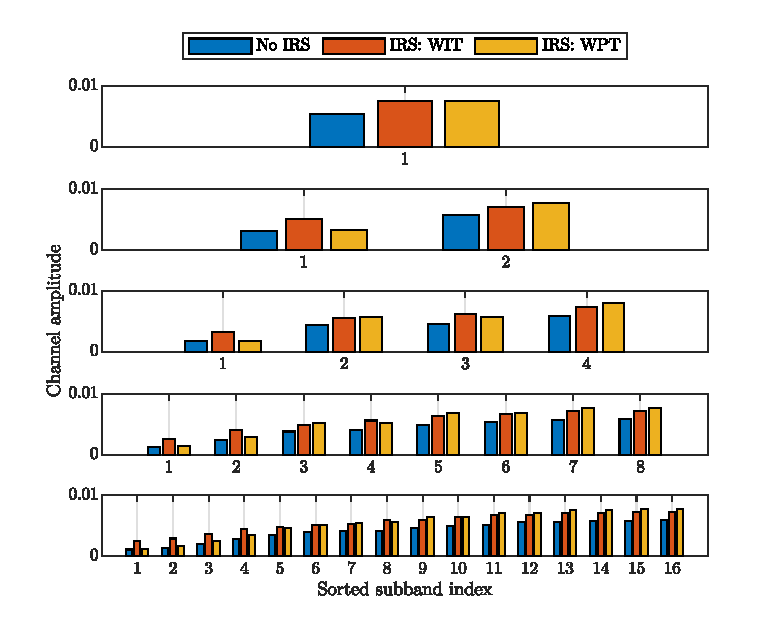
\includegraphics{../assets/channel_amplitude}
				}
				\caption{Channel amplitude with and without IRS versus $N$ for $M=1$, $L=100$, $\sigma_n^2=\SI{-40}{\dBm}$, $B=\SI{10}{\MHz}$ and $d_{\mathrm{H}}=d_{\mathrm{V}}=\SI{2}{\meter}$.}
				\label{fi:channel_amplitude}
			\end{figure}

			On the other hand, the corresponding amplitude of modulated and multisine waveforms are shown in Fig.~\ref{fi:waveform_amplitude}. Note that no multisine is used for WIT and the case is not shown. It is observed that although passive beamforming can enable a flexible resource allocation opportunity at the channel (please refer to Response~\ref{re:2.10} for details), its impact on waveform design is unobvious.

			\begin{figure}[!h]
				\centering
				\subfloat[WIT waveform: modulated]{
				\resizebox{0.32\columnwidth}{!}{
						% This file was created by matlab2tikz.
%
%The latest updates can be retrieved from
%  http://www.mathworks.com/matlabcentral/fileexchange/22022-matlab2tikz-matlab2tikz
%where you can also make suggestions and rate matlab2tikz.
%
\definecolor{mycolor1}{rgb}{0.00000,0.44700,0.74100}%
\definecolor{mycolor2}{rgb}{0.85000,0.32500,0.09800}%
%
\begin{tikzpicture}

\begin{axis}[%
width=4.036in,
height=0.429in,
at={(0.677in,3.242in)},
scale only axis,
xmin=0,
xmax=2,
xtick={1},
ymin=0,
ymax=4.47213595499958,
ytick={0, 2, 4},
axis background/.style={fill=white},
xmajorgrids,
ymajorgrids,
legend style={at={(0.5,1.03)}, anchor=south, legend columns=2, legend cell align=left, align=left, draw=white!15!black},
title style={font=\huge}, label style={font=\huge}, ticklabel style={font=\LARGE}, legend style={font=\LARGE}
]
\addplot[ycomb, color=mycolor1, line width=2.0pt, mark=o, mark options={solid, mycolor1}] table[row sep=crcr] {%
1	4.47213595499958\\
};
\addplot[forget plot, color=white!15!black, line width=2.0pt] table[row sep=crcr] {%
0	0\\
2	0\\
};
\addlegendentry{IRS: {\boldmath${s}$}$_{\mathrm{I}}$}

\addplot[ycomb, color=mycolor2, line width=2.0pt, mark=x, mark options={solid, mycolor2}] table[row sep=crcr] {%
1	4.47213595499958\\
};
\addplot[forget plot, color=white!15!black, line width=2.0pt] table[row sep=crcr] {%
0	0\\
2	0\\
};
\addlegendentry{No IRS: {\boldmath${s}$}$_{\mathrm{I}}$}

\end{axis}

\begin{axis}[%
width=4.036in,
height=0.429in,
at={(0.677in,2.546in)},
scale only axis,
xmin=0,
xmax=3,
xtick={1, 2},
ymin=0,
ymax=4.47213595499958,
ytick={0, 2, 4},
axis background/.style={fill=white},
xmajorgrids,
ymajorgrids,
title style={font=\huge}, label style={font=\huge}, ticklabel style={font=\LARGE}, legend style={font=\LARGE}
]
\addplot[ycomb, color=mycolor1, line width=2.0pt, mark=o, mark options={solid, mycolor1}, forget plot] table[row sep=crcr] {%
1	3.16197544010622\\
2	3.16257985135002\\
};
\addplot[forget plot, color=white!15!black, line width=2.0pt] table[row sep=crcr] {%
0	0\\
3	0\\
};
\addplot[ycomb, color=mycolor2, line width=2.0pt, mark=x, mark options={solid, mycolor2}, forget plot] table[row sep=crcr] {%
1	3.16115798980538\\
2	3.16339693422903\\
};
\addplot[forget plot, color=white!15!black, line width=2.0pt] table[row sep=crcr] {%
0	0\\
3	0\\
};
\end{axis}

\begin{axis}[%
width=4.036in,
height=0.429in,
at={(0.677in,1.85in)},
scale only axis,
xmin=0,
xmax=5,
xtick={1, 2, 3, 4},
ymin=0,
ymax=4.47213595499958,
ytick={0, 2, 4},
ylabel style={font=\color{white!15!black}},
ylabel={Waveform amplitude},
axis background/.style={fill=white},
xmajorgrids,
ymajorgrids,
title style={font=\huge}, label style={font=\huge}, ticklabel style={font=\LARGE}, legend style={font=\LARGE}
]
\addplot[ycomb, color=mycolor1, line width=2.0pt, mark=o, mark options={solid, mycolor1}, forget plot] table[row sep=crcr] {%
1	2.23378952118842\\
2	2.23654464483002\\
3	2.23679993610816\\
4	2.23713622127432\\
};
\addplot[forget plot, color=white!15!black, line width=2.0pt] table[row sep=crcr] {%
0	0\\
5	0\\
};
\addplot[ycomb, color=mycolor2, line width=2.0pt, mark=x, mark options={solid, mycolor2}, forget plot] table[row sep=crcr] {%
1	2.22545319620151\\
2	2.23919103086275\\
3	2.23937811584463\\
4	2.24021589430493\\
};
\addplot[forget plot, color=white!15!black, line width=2.0pt] table[row sep=crcr] {%
0	0\\
5	0\\
};
\end{axis}

\begin{axis}[%
width=4.036in,
height=0.429in,
at={(0.677in,1.154in)},
scale only axis,
xmin=0,
xmax=9,
xtick={1, 2, 3, 4, 5, 6, 7, 8},
ymin=0,
ymax=4.47213595499958,
ytick={0, 2, 4},
axis background/.style={fill=white},
xmajorgrids,
ymajorgrids,
title style={font=\huge}, label style={font=\huge}, ticklabel style={font=\LARGE}, legend style={font=\LARGE}
]
\addplot[ycomb, color=mycolor1, line width=2.0pt, mark=o, mark options={solid, mycolor1}, forget plot] table[row sep=crcr] {%
1	1.57492536161738\\
2	1.58019558798915\\
3	1.58142030797172\\
4	1.58199169722726\\
5	1.58244513043393\\
6	1.58255247448636\\
7	1.58277901011216\\
8	1.58278544606781\\
};
\addplot[forget plot, color=white!15!black, line width=2.0pt] table[row sep=crcr] {%
0	0\\
9	0\\
};
\addplot[ycomb, color=mycolor2, line width=2.0pt, mark=x, mark options={solid, mycolor2}, forget plot] table[row sep=crcr] {%
1	1.54658301793324\\
2	1.57890604600973\\
3	1.58567053153604\\
4	1.58602764687811\\
5	1.58742152113889\\
6	1.58776504632019\\
7	1.58809335949322\\
8	1.5881928373826\\
};
\addplot[forget plot, color=white!15!black, line width=2.0pt] table[row sep=crcr] {%
0	0\\
9	0\\
};
\end{axis}

\begin{axis}[%
width=4.036in,
height=0.429in,
at={(0.677in,0.458in)},
scale only axis,
xmin=0,
xmax=17,
xtick={ 1,  2,  3,  4,  5,  6,  7,  8,  9, 10, 11, 12, 13, 14, 15, 16},
xlabel style={font=\color{white!15!black}},
xlabel={Sorted subband index},
ymin=0,
ymax=4.47213595499958,
ytick={0, 2, 4},
axis background/.style={fill=white},
xmajorgrids,
ymajorgrids,
title style={font=\huge}, label style={font=\huge}, ticklabel style={font=\LARGE}, legend style={font=\LARGE}
]
\addplot[ycomb, color=mycolor1, line width=2.0pt, mark=o, mark options={solid, mycolor1}, forget plot] table[row sep=crcr] {%
1	1.10693759886133\\
2	1.11152957304454\\
3	1.1153740214668\\
4	1.11770662066146\\
5	1.11834620668734\\
6	1.11879936603067\\
7	1.11890444505621\\
8	1.11953756000214\\
9	1.11961027059849\\
10	1.1199195311366\\
11	1.12011494881618\\
12	1.12017416958603\\
13	1.12033284686217\\
14	1.12033895948864\\
15	1.12040846172897\\
16	1.12041390652564\\
};
\addplot[forget plot, color=white!15!black, line width=2.0pt] table[row sep=crcr] {%
0	0\\
17	0\\
};
\addplot[ycomb, color=mycolor2, line width=2.0pt, mark=x, mark options={solid, mycolor2}, forget plot] table[row sep=crcr] {%
1	1.05608889731275\\
2	1.08431501210806\\
3	1.10834050856176\\
4	1.11891055117252\\
5	1.12321530567299\\
6	1.12470216682288\\
7	1.12523793678797\\
8	1.12552298915589\\
9	1.12642268676024\\
10	1.12689100352585\\
11	1.127202079253\\
12	1.12763006638833\\
13	1.12766695997673\\
14	1.12788476342969\\
15	1.1278991085713\\
16	1.12794901573584\\
};
\addplot[forget plot, color=white!15!black, line width=2.0pt] table[row sep=crcr] {%
0	0\\
17	0\\
};
\end{axis}
\end{tikzpicture}%
					}
				}
				\subfloat[WPT waveform: modulated]{
					\resizebox{0.32\columnwidth}{!}{
						% This file was created by matlab2tikz.
%
%The latest updates can be retrieved from
%  http://www.mathworks.com/matlabcentral/fileexchange/22022-matlab2tikz-matlab2tikz
%where you can also make suggestions and rate matlab2tikz.
%
\definecolor{mycolor1}{rgb}{0.00000,0.44700,0.74100}%
\definecolor{mycolor2}{rgb}{0.85000,0.32500,0.09800}%
%
\begin{tikzpicture}

\begin{axis}[%
width=4.036in,
height=0.42in,
at={(0.677in,3.251in)},
scale only axis,
xmin=0,
xmax=2,
xtick={1},
ymin=0,
ymax=5,
ytick={0, 2, 4},
axis background/.style={fill=white},
xmajorgrids,
ymajorgrids,
legend style={at={(0.5,1.03)}, anchor=south, legend columns=2, legend cell align=left, align=left, draw=white!15!black},
title style={font=\large}, label style={font=\large}, ticklabel style={font=\large}, legend style={font=\large}
]
\addplot[ycomb, color=mycolor1, line width=2.0pt, mark=o, mark options={solid, mycolor1}] table[row sep=crcr] {%
1	4.47213595034367\\
};
\addplot[forget plot, color=white!15!black, line width=2.0pt] table[row sep=crcr] {%
0	0\\
2	0\\
};
\addlegendentry{IRS: {\boldmath${s}$}$_{\mathrm{I}}$}

\addplot[ycomb, color=mycolor2, line width=2.0pt, mark=x, mark options={solid, mycolor2}] table[row sep=crcr] {%
1	4.47213593685897\\
};
\addplot[forget plot, color=white!15!black, line width=2.0pt] table[row sep=crcr] {%
0	0\\
2	0\\
};
\addlegendentry{No IRS: {\boldmath${s}$}$_{\mathrm{I}}$}

\end{axis}

\begin{axis}[%
width=4.036in,
height=0.42in,
at={(0.677in,2.553in)},
scale only axis,
xmin=0,
xmax=3,
xtick={1, 2},
ymin=0,
ymax=5,
ytick={0, 2, 4},
axis background/.style={fill=white},
xmajorgrids,
ymajorgrids,
title style={font=\large}, label style={font=\large}, ticklabel style={font=\large}, legend style={font=\large}
]
\addplot[ycomb, color=mycolor1, line width=2.0pt, mark=o, mark options={solid, mycolor1}, forget plot] table[row sep=crcr] {%
1	0.000570870326956724\\
2	4.4721359179404\\
};
\addplot[forget plot, color=white!15!black, line width=2.0pt] table[row sep=crcr] {%
0	0\\
3	0\\
};
\addplot[ycomb, color=mycolor2, line width=2.0pt, mark=x, mark options={solid, mycolor2}, forget plot] table[row sep=crcr] {%
1	0.0110856763978608\\
2	4.47212221176042\\
};
\addplot[forget plot, color=white!15!black, line width=2.0pt] table[row sep=crcr] {%
0	0\\
3	0\\
};
\end{axis}

\begin{axis}[%
width=4.036in,
height=0.42in,
at={(0.677in,1.855in)},
scale only axis,
xmin=0,
xmax=5,
xtick={1, 2, 3, 4},
ymin=0,
ymax=5,
ytick={0, 2, 4},
ylabel style={font=\color{white!15!black}},
ylabel={Waveform amplitude},
axis background/.style={fill=white},
xmajorgrids,
ymajorgrids,
title style={font=\large}, label style={font=\large}, ticklabel style={font=\large}, legend style={font=\large}
]
\addplot[ycomb, color=mycolor1, line width=2.0pt, mark=o, mark options={solid, mycolor1}, forget plot] table[row sep=crcr] {%
1	1.82810775851695e-05\\
2	3.53085892593064e-05\\
3	3.54347120351704e-05\\
4	4.42555930751421\\
};
\addplot[forget plot, color=white!15!black, line width=2.0pt] table[row sep=crcr] {%
0	0\\
5	0\\
};
\addplot[ycomb, color=mycolor2, line width=2.0pt, mark=x, mark options={solid, mycolor2}, forget plot] table[row sep=crcr] {%
1	1.22676166428777e-05\\
2	2.19662118918467e-05\\
3	2.35611473414708e-05\\
4	4.38314990531919\\
};
\addplot[forget plot, color=white!15!black, line width=2.0pt] table[row sep=crcr] {%
0	0\\
5	0\\
};
\end{axis}

\begin{axis}[%
width=4.036in,
height=0.42in,
at={(0.677in,1.157in)},
scale only axis,
xmin=0,
xmax=9,
xtick={1, 2, 3, 4, 5, 6, 7, 8},
ymin=0,
ymax=1,
ytick={0, 1},
axis background/.style={fill=white},
xmajorgrids,
ymajorgrids,
title style={font=\large}, label style={font=\large}, ticklabel style={font=\large}, legend style={font=\large}
]
\addplot[ycomb, color=mycolor1, line width=2.0pt, mark=o, mark options={solid, mycolor1}, forget plot] table[row sep=crcr] {%
1	6.25263040326118e-06\\
2	6.27921380470113e-06\\
3	6.34955721457943e-06\\
4	6.35150273149039e-06\\
5	6.42390701416729e-06\\
6	6.42457974220412e-06\\
7	6.47741859691329e-06\\
8	6.47969375628299e-06\\
};
\addplot[forget plot, color=white!15!black, line width=2.0pt] table[row sep=crcr] {%
0	0\\
9	0\\
};
\addplot[ycomb, color=mycolor2, line width=2.0pt, mark=x, mark options={solid, mycolor2}, forget plot] table[row sep=crcr] {%
1	2.07597912435039e-05\\
2	2.10621157490525e-05\\
3	2.27177871268911e-05\\
4	2.34764127724776e-05\\
5	0.000633429285281999\\
6	0.00299168089473067\\
7	0.0168627108170759\\
8	0.0302609478988545\\
};
\addplot[forget plot, color=white!15!black, line width=2.0pt] table[row sep=crcr] {%
0	0\\
9	0\\
};
\end{axis}

\begin{axis}[%
width=4.036in,
height=0.42in,
at={(0.677in,0.458in)},
scale only axis,
xmin=0,
xmax=17,
xtick={ 1,  2,  3,  4,  5,  6,  7,  8,  9, 10, 11, 12, 13, 14, 15, 16},
xlabel style={font=\color{white!15!black}},
xlabel={Sorted subband index},
ymin=0,
ymax=1,
ytick={0, 1},
axis background/.style={fill=white},
xmajorgrids,
ymajorgrids,
title style={font=\large}, label style={font=\large}, ticklabel style={font=\large}, legend style={font=\large}
]
\addplot[ycomb, color=mycolor1, line width=2.0pt, mark=o, mark options={solid, mycolor1}, forget plot] table[row sep=crcr] {%
1	1.46841221768753e-06\\
2	1.46853581584948e-06\\
3	1.46888556831603e-06\\
4	1.46960879811052e-06\\
5	1.47063822579491e-06\\
6	1.47112726920342e-06\\
7	1.47158812622008e-06\\
8	1.47177039924161e-06\\
9	1.47273523214333e-06\\
10	1.47288042283048e-06\\
11	1.47389962773962e-06\\
12	1.47396082891411e-06\\
13	1.47467419234042e-06\\
14	1.47476166458671e-06\\
15	1.47506643379659e-06\\
16	1.47509099313304e-06\\
};
\addplot[forget plot, color=white!15!black, line width=2.0pt] table[row sep=crcr] {%
0	0\\
17	0\\
};
\addplot[ycomb, color=mycolor2, line width=2.0pt, mark=x, mark options={solid, mycolor2}, forget plot] table[row sep=crcr] {%
1	1.08632407458004e-05\\
2	1.08877007745949e-05\\
3	1.09594364217047e-05\\
4	1.10938027865036e-05\\
5	1.12827891666553e-05\\
6	1.15378065652616e-05\\
7	1.19617266900702e-05\\
8	1.41613520483063e-05\\
9	6.92466622068608e-05\\
10	0.000224790946436711\\
11	0.000536194940235116\\
12	0.0020179447121528\\
13	0.00228142595005787\\
14	0.00484194141261625\\
15	0.00509975660438143\\
16	0.00611499201390601\\
};
\addplot[forget plot, color=white!15!black, line width=2.0pt] table[row sep=crcr] {%
0	0\\
17	0\\
};
\end{axis}
\end{tikzpicture}%
					}
				}
				\subfloat[WPT waveform: multisine]{
					\resizebox{0.32\columnwidth}{!}{
						% This file was created by matlab2tikz.
%
%The latest updates can be retrieved from
%  http://www.mathworks.com/matlabcentral/fileexchange/22022-matlab2tikz-matlab2tikz
%where you can also make suggestions and rate matlab2tikz.
%
\definecolor{mycolor1}{rgb}{0.00000,0.44700,0.74100}%
\definecolor{mycolor2}{rgb}{0.85000,0.32500,0.09800}%
%
\begin{tikzpicture}

\begin{axis}[%
width=3.972in,
height=0.503in,
at={(0.666in,3.312in)},
scale only axis,
xmin=0,
xmax=2,
xtick={1},
ymin=0,
ymax=4.47213595499958,
axis background/.style={fill=white},
xmajorgrids,
ymajorgrids,
legend style={legend cell align=left, align=left, draw=white!15!black},
title style={font=\huge}, label style={font=\huge}, ticklabel style={font=\LARGE}, legend style={font=\LARGE}
]
\addplot[ycomb, color=mycolor1, line width=2.0pt, mark=o, mark options={solid, mycolor1}] table[row sep=crcr] {%
1	0.000331092582051402\\
};
\addplot[forget plot, color=white!15!black, line width=2.0pt] table[row sep=crcr] {%
0	0\\
2	0\\
};
\addlegendentry{IRS: {\boldmath${s}$}$_{\mathrm{P}}$}

\addplot[ycomb, color=mycolor2, line width=2.0pt, mark=x, mark options={solid, mycolor2}] table[row sep=crcr] {%
1	0.000301200841788861\\
};
\addplot[forget plot, color=white!15!black, line width=2.0pt] table[row sep=crcr] {%
0	0\\
2	0\\
};
\addlegendentry{No IRS: {\boldmath${s}$}$_{\mathrm{P}}$}

\end{axis}

\begin{axis}[%
width=3.972in,
height=0.503in,
at={(0.666in,2.598in)},
scale only axis,
xmin=0,
xmax=3,
xtick={1, 2},
ymin=0,
ymax=4.47213595499958,
axis background/.style={fill=white},
xmajorgrids,
ymajorgrids,
title style={font=\huge}, label style={font=\huge}, ticklabel style={font=\LARGE}, legend style={font=\LARGE}
]
\addplot[ycomb, color=mycolor1, line width=2.0pt, mark=o, mark options={solid, mycolor1}, forget plot] table[row sep=crcr] {%
1	8.31476170438795e-06\\
2	8.59623838841982e-06\\
};
\addplot[forget plot, color=white!15!black, line width=2.0pt] table[row sep=crcr] {%
0	0\\
3	0\\
};
\addplot[ycomb, color=mycolor2, line width=2.0pt, mark=x, mark options={solid, mycolor2}, forget plot] table[row sep=crcr] {%
1	2.51350625686209e-05\\
2	2.5738452816653e-05\\
};
\addplot[forget plot, color=white!15!black, line width=2.0pt] table[row sep=crcr] {%
0	0\\
3	0\\
};
\end{axis}

\begin{axis}[%
width=3.972in,
height=0.503in,
at={(0.666in,1.883in)},
scale only axis,
xmin=0,
xmax=5,
xtick={1, 2, 3, 4},
ymin=0,
ymax=4.47213595499958,
ylabel style={font=\color{white!15!black}},
ylabel={Waveform amplitude},
axis background/.style={fill=white},
xmajorgrids,
ymajorgrids,
title style={font=\huge}, label style={font=\huge}, ticklabel style={font=\LARGE}, legend style={font=\LARGE}
]
\addplot[ycomb, color=mycolor1, line width=2.0pt, mark=o, mark options={solid, mycolor1}, forget plot] table[row sep=crcr] {%
1	1.81401011150761e-05\\
2	7.63567990520219e-05\\
3	0.000347720308108743\\
4	1.20961154306659\\
};
\addplot[forget plot, color=white!15!black, line width=2.0pt] table[row sep=crcr] {%
0	0\\
5	0\\
};
\addplot[ycomb, color=mycolor2, line width=2.0pt, mark=x, mark options={solid, mycolor2}, forget plot] table[row sep=crcr] {%
1	0.00111014489403298\\
2	0.00243652079053788\\
3	0.00358274270606404\\
4	1.61181535442991\\
};
\addplot[forget plot, color=white!15!black, line width=2.0pt] table[row sep=crcr] {%
0	0\\
5	0\\
};
\end{axis}

\begin{axis}[%
width=3.972in,
height=0.503in,
at={(0.666in,1.168in)},
scale only axis,
xmin=0,
xmax=9,
xtick={1, 2, 3, 4, 5, 6, 7, 8},
ymin=0,
ymax=4.47213595499958,
axis background/.style={fill=white},
xmajorgrids,
ymajorgrids,
title style={font=\huge}, label style={font=\huge}, ticklabel style={font=\LARGE}, legend style={font=\LARGE}
]
\addplot[ycomb, color=mycolor1, line width=2.0pt, mark=o, mark options={solid, mycolor1}, forget plot] table[row sep=crcr] {%
1	0.406193755485101\\
2	0.6086191375554\\
3	0.70781380097226\\
4	1.11700551493449\\
5	1.39413019214519\\
6	1.89924922357725\\
7	2.27606557910904\\
8	2.64280256661518\\
};
\addplot[forget plot, color=white!15!black, line width=2.0pt] table[row sep=crcr] {%
0	0\\
9	0\\
};
\addplot[ycomb, color=mycolor2, line width=2.0pt, mark=x, mark options={solid, mycolor2}, forget plot] table[row sep=crcr] {%
1	0.621345098069754\\
2	0.710296651693143\\
3	0.908023988477654\\
4	1.12050035456782\\
5	1.44244708781013\\
6	1.77492365099369\\
7	2.30702814170141\\
8	2.53638471775812\\
};
\addplot[forget plot, color=white!15!black, line width=2.0pt] table[row sep=crcr] {%
0	0\\
9	0\\
};
\end{axis}

\begin{axis}[%
width=3.972in,
height=0.503in,
at={(0.666in,0.454in)},
scale only axis,
xmin=0,
xmax=17,
xtick={ 1,  2,  3,  4,  5,  6,  7,  8,  9, 10, 11, 12, 13, 14, 15, 16},
xlabel style={font=\color{white!15!black}},
xlabel={Sorted subband index},
ymin=0,
ymax=4.47213595499958,
axis background/.style={fill=white},
xmajorgrids,
ymajorgrids,
title style={font=\huge}, label style={font=\huge}, ticklabel style={font=\LARGE}, legend style={font=\LARGE}
]
\addplot[ycomb, color=mycolor1, line width=2.0pt, mark=o, mark options={solid, mycolor1}, forget plot] table[row sep=crcr] {%
1	0.280439553353647\\
2	0.384605443069534\\
3	0.416114603863305\\
4	0.499024317224016\\
5	0.571268128602638\\
6	0.621900186283823\\
7	0.763344617968865\\
8	0.858693319856245\\
9	0.954356161751161\\
10	1.16907743761735\\
11	1.21561270661726\\
12	1.45089690540298\\
13	1.51204499963039\\
14	1.68681223326519\\
15	1.74569476977388\\
16	1.81071246294588\\
};
\addplot[forget plot, color=white!15!black, line width=2.0pt] table[row sep=crcr] {%
0	0\\
17	0\\
};
\addplot[ycomb, color=mycolor2, line width=2.0pt, mark=x, mark options={solid, mycolor2}, forget plot] table[row sep=crcr] {%
1	0.447567787711277\\
2	0.504906671531525\\
3	0.589458291557858\\
4	0.619646960375962\\
5	0.691059903147371\\
6	0.741736916016998\\
7	0.810826698348076\\
8	0.887751406400927\\
9	0.941910732226763\\
10	1.15698606523739\\
11	1.20259880483264\\
12	1.42353667332449\\
13	1.46532152628089\\
14	1.65027292091107\\
15	1.65828648619566\\
16	1.73730645060792\\
};
\addplot[forget plot, color=white!15!black, line width=2.0pt] table[row sep=crcr] {%
0	0\\
17	0\\
};
\end{axis}
\end{tikzpicture}%
					}
				}
				\caption{Sorted modulated and multisine amplitude for WIT and WPT with and without IRS versus $N$ for $M=1$, $L=20$, $\sigma_n^2=\SI{-40}{\dBm}$, $B=\SI{10}{\MHz}$ and $d_{\mathrm{H}}=d_{\mathrm{V}}=\SI{2}{\meter}$.}
				\label{fi:waveform_amplitude}
			\end{figure}

			We have modified the manuscript as follows to emphasize this point.
			\begin{framed}
				Fig.~\ref{M-fi:channel_amplitude} reveals how IRS influences the (sorted) channel amplitude and waveform design for one channel realization. Thanks to the flexible subchannel design enabled by passive beamforming, the optimal subchannel strength distribution for WIT and WPT are dissimilar. Under the specified configuration, the WPT-optimized IRS aligns the strong subbands to exploit the rectifier nonlinearity. On the other hand, the WIT-optimized IRS provides a fair gain over all subchannels when $L$ is sufficiently large. This is reminiscent of the water-filling scheme at high SNR, but is realized by channel alignment instead of resource allocation. Moreover, the amplitude of modulated and multisine waveforms with and without IRS are shown in Figs.~\ref{M-fi:waveform_wit_modulated}--\ref{M-fi:waveform_wpt_multisine}.\footnotemark It is concluded that adding an IRS to the SWIPT system has subtle impact on the waveform design.
			\end{framed}
			\footnotetext{Note that no multisine is used for WIT and the case is not shown.}
			\label{re:2.2}
		\end{response}

		\begin{point}
			In the introduction, it is suggested to also discuss the new design challenges posed by the nonlinear model compared to the existing designs under the linear model.
		\end{point}

		\begin{response}
			We believe this is an important issue and have modified the manuscript accordingly as follows.
			\begin{framed}
				Although this tractable harvester model accurately reveals how the input power level and waveform shape influence the output DC power, it also introduces design challenges such as frequency coupling (i.e., components of different frequencies compensate and produce DC), waveform coupling (i.e., different waveforms jointly contribute to DC), and high-order objective function.
			\end{framed}
			\label{re:2.3}
		\end{response}

		\begin{point}
			In \ref{M-op:original}, the authors integrated the waveform design and active beamforming design into $\boldsymbol{w}_{\mathrm{I}}$ and $\boldsymbol{w}_{\mathrm{P}}$. However, they separately optimized them later. Is it possible to directly optimize $\boldsymbol{w}_{\mathrm{I}}$ and $\boldsymbol{w}_{\mathrm{P}}$ as a whole?
		\end{point}

		\begin{response}
			For the single-user case, direct optimization on $\boldsymbol{w}_{\mathrm{I}}$ and $\boldsymbol{w}_{\mathrm{P}}$ is possible. The reviewer is referred to Algorithm 1 of \cite{M-Clerckx2018b} for more details, and the idea is briefly described as follows. First, $\boldsymbol{w}_{\mathrm{I}}$ and $\boldsymbol{w}_{\mathrm{P}}$ are complex variables of size $MN \times 1$. To enable GP tools (which apply to problems involving real-valued variables), we notice that the optimal phase of $\boldsymbol{w}_{\mathrm{I}}$ and $\boldsymbol{w}_{\mathrm{P}}$ should be designed to compensate the phase of the corresponding composite channel $\boldsymbol{h}$, namely
			\begin{equation}
				\arg(\boldsymbol{w}_{\mathrm{I}}) = \arg(\boldsymbol{w}_{\mathrm{P}}) = -\arg(\boldsymbol{h}),
			\end{equation}
			such that, from the perspective of phase design, the current expression \ref{M-eq:z_expand} is maximized (where all $\cos$ terms peak at \num{1}) and the rate expression is maximized (where the phases align with those of matched filters). Therefore, the direct optimization on $\boldsymbol{w}_{\mathrm{I}}$ and $\boldsymbol{w}_{\mathrm{P}}$ boils down to amplitude optimization on $\boldsymbol{s}_{\mathrm{I}}$ and $\boldsymbol{s}_{\mathrm{P}}$, where $\boldsymbol{s}_{\mathrm{I/P}}=\lvert \boldsymbol{w}_{\mathrm{I/P}} \rvert$. GP tools can be applied at this stage and the number of real-valued variables are $2MN$. In contrast, the proposed design decouples the design in the spatial and frequency domains, derives the global optimal active precoder, and leaves a resource allocation issue with $2N$ real-valued variables in the frequency domain. Since the computational complexity of GP scales exponentially with the number of variables, optimizing $\boldsymbol{w}_{\mathrm{I}}$ and $\boldsymbol{w}_{\mathrm{P}}$ as a whole can be very inefficient and not discussed in the manuscript. Accordingly, we have revised the manuscript as follows.
			\begin{framed}
				To avoid straightforward optimization over complex vectors $\boldsymbol{w}_{\mathrm{I/P}}$ of size $MN \times 1$, we decouple the waveform in the spatial and frequency domains to reduce the size of variables.
			\end{framed}
		\end{response}

		\begin{point}
			In the low-complexity BCD, it is unclear how the authors dealt with the optimization of $\rho$ and $\delta$. In Algorithm~\ref{M-al:lc_bcd}, both of them are input. Did the authors perform a two-dimensional search here? Besides, they were assumed to be identical in the simulation. How will this assumption influence the performance loss?
		\end{point}

		\begin{response}
			Thank you for raising this point. The combining ratio $\delta$ determines the priority on multisine power waveform at the transmitter, while the splitting ratio $\rho$ determines the priority of the energy harvester at the receiver. We notice that $\delta^{\star}=\rho^{\star}=0$ at the WIT point and $\delta^{\star}=\rho^{\star}=1$ at the WPT point when $N$ is relatively large. Heuristically, $\delta$ and $\rho$ should approximately equal at each point to boost R-E tradeoff. Indeed, the LC-BCD algorithm intends to draw the R-E tradeoff by performing a two-dimensional search that adjusts $\delta$ and $\rho$ from \num{0} to \num{1}. However, based on the deduction above, we set $\delta=\rho$ is the simulation and obtain the R-E region by one-dimensional search instead. The results show that even a one-dimensional search for the LC-BCD algorithm can achieve a very good performance. We have summarized the point in the manuscript as follows.
			\begin{framed}
				\textellipsis where the combining ratio $\delta$ determines the priority on multisine power waveform at the transmitter and the splitting ratio $\rho$ determines the priority of the energy harvester at the receiver\footnotemark.

				\textellipsis Note that the BCD algorithm obtains the R-E region by varying the rate constraint from \num{0} to maximum capacity $C_{\max}$, while the LC-BCD algorithm obtains the R-E region by two-dimensional search over $\{\delta,\rho\}$ from \num{0} to \num{1}.

				\textellipsis assume $\delta=\rho$ for simplicity (thus one-dimensional search to obtain the R-E region).

				\textellipsis  Besides, the LC-BCD algorithm achieves a good balance between performance and complexity even if one-dimensional search is considered for $\delta=\rho$ from \num{0} to \num{1}.
			\end{framed}
			\footnotetext{We notice that $\delta^{\star}=\rho^{\star}=0$ at the WIT point and $\delta^{\star}=\rho^{\star}=1$ at the WPT point when $N$ is relatively large. Heuristically, $\delta^{\star}$ and $\rho^{\star}$ should approximately equal at each point to boost R-E tradeoff.}
		\end{response}

		\begin{point}
			If possible, in Figs.~\ref{M-fi:re_irs_1mhz} and \ref{M-fi:re_irs_10mhz}, the authors can show the performance of the design under the conventional linear harvester model, so as to show how much performance loss it would incur.
		\end{point}

		\begin{response}
			We would like to clarify that the performance loss under the conventional linear harvester model is revealed instead in Figs.~\ref{M-fi:scaling_tx} and \ref{M-fi:scaling_reflector}. Figs.~\ref{M-fi:re_irs_1mhz} and \ref{M-fi:re_irs_10mhz} are intended to compare different IRS strategies when both waveform and passive beamforming are designed under nonlinear harvester model. The authors believe that to design passive beamforming under linear harvester model when the waveform is designed under nonlinear harvester model might confuse the readers. On the other hand, we agree with the reviewer that the performance loss under linear harvester deserves more attention, and have changed the label in Figs.~\ref{M-fi:scaling_tx} and \ref{M-fi:scaling_reflector} from `ASS' to `LEH' and revised the manuscript as follows to make this point clear.
			\begin{framed}
				Second, the conventional Linear Energy Harvester (LEH) model leads to a power-inefficient design. To investigate the performance loss, we truncate the DC objective function \eqref{M-eq:z} at $n_0=2$ such that 1) in the passive beamforming problem, $z(\boldsymbol{\Phi}) = {\beta_2}{\rho}(t_{\mathrm{I},0}+t_{\mathrm{P},0})/2$ and no SCA is required; 2) in the waveform design problem, the WPT-optimal strategy is the Adaptive Single Sinewave (ASS) waveform strategy that allocates all power to the multisine at the strongest subband \cite{M-Clerckx2016a}. As shown in Figs.~\ref{M-fi:scaling_tx} and \ref{M-fi:scaling_reflector}, those conventional designs do not exploit the harvester nonlinearity and end up with a nearly \SI{20}{\dB} gap compared to the nonlinear model-based SMF and GP designs.
			\end{framed}
		\end{response}

		\begin{point}
			It was shown via simulation that PS is not always superior to TS, unlike the linear model. Is it possible to develop some analytical preconditions to determine which one is better?
		\end{point}

		\begin{response}
			We concluded that PS outperforms TS when the number of subcarrier is relatively small or when the SNR is relatively large. However, the analytical preconditions in the proposed system can be very hard to obtain because SNR can depend on many factors (e.g., distance of all paths, number of IRS elements, average noise power, etc.). Essentially, this behavior origins from the waveform selection and we would like to analyze it in a nutshell.

			TS only performs a naive time-sharing between the WIT point and the WPT point. At the WIT point, only modulated waveform is used to maximize the achievable rate. At the WPT point, the optimal waveform depends on the number of subcarriers $N$. Although the modulated waveform has an modulation gain of \num{2} that outstands for a small $N$, it creates no DC coupling between frequencies and is outperformed by multisine for a large $N$. Therefore, for a relatively small $N$, the modulated waveform is used at both WIT and WPT point, and one can heuristically infer that no multisine waveform is needed for any point (this is verified in simulation). In this case, the R-E region is convex, which aligns with the conventional linear harvester model (PS outperforms TS and dedicated power waveform is unnecessary). However, as $N$ becomes sufficiently large, multisine waveform further boosts the WPT point due to its power benefit under nonlinear harvester model. It creates some concavity in the high-power region and accounts for the superiority of TS.

			Similar effect exists for SNR. At high SNR, the SWIPT user can achieve a decent rate even if a small fraction of transmit power is allocated to the modulated waveform. Therefore, one can approach high-rate region fast at a small cost of DC power at high SNR. This is however impossible at low SNR.

			The manuscript has been updated as follows.
			\begin{framed}
				Second, the R-E region is convex for $N \in \{2,4\}$ and concave-convex for $N \in \{8,16\}$, such that PS outperforms TS for a small $N$ and is outperformed for a large $N$. When $N$ is in between, the optimal strategy is a combination of both, i.e., a time sharing between the WPT point and the saddle PS SWIPT point (as denoted by the red curve in Fig.~\ref{M-fi:re_subband}). When $N$ is relatively small, only modulated waveform is used at both WIT and WPT point, and one can infer that no multisine waveform is needed for the entire R-E region. It aligns with the conclusion based on conventional linear harvester model, namely the R-E region is convex, PS outperforms TS, and dedicated power waveform is unnecessary. As $N$ becomes sufficiently large, multisine waveform further boosts WPT and creates some concavity in the high-power region, which accounts for the superiority of TS under nonlinear harvester model. Therefore, we conclude that the rectifier nonlinearity enlarges the R-E region by favoring a different waveform and receiving mode, both heavily depending on $N$.
			\end{framed}
		\end{response}

		\begin{point}
			Is it possible to give the complexity order of the algorithms presented in this paper?
		\end{point}

		\begin{response}
			We have added complexity analysis in the revised manuscript. The reviewer is referred to Response~\ref{re:1.1} for details.
		\end{response}

		\begin{point}
			The expressions of signals in (1), (2), and (5) are not conventional. It may be better to give a per-band signal instead of their superposition. Besides, it is better to first introduce the functionalities of the modulated and multisine waveforms before giving (1).
		\end{point}

		\begin{response}
			We agree with the reviewer that the signal model requires more description. The manuscript has been updated as follows.
			\begin{framed}
				As suggested in \cite{M-Clerckx2018b}, we superpose a multi-carrier modulated information-bearing waveform to a multi-carrier unmodulated power-dedicated waveform (deterministic multisine) to boost the spectrum and energy efficiency. The information signal transmitted over subband $n \in \mathcal{N} \triangleq \{1, \dots, N\}$ at time $t$ is
				\begin{equation}
					\boldsymbol{x}_{\mathrm{I},n}(t) = \Re\left\{\boldsymbol{w}_{\mathrm{I},n} \tilde{x}_{\mathrm{I},n}(t) e^{j2{\pi}{f_n}{t}}\right\},
				\end{equation}
				where $\boldsymbol{w}_{\mathrm{I},n} \in \mathbb{C}^{M \times 1}$ is the information precoder at subband $n$, $\tilde{x}_{\mathrm{I},n}\sim\mathcal{CN}(0,1)$ is the information symbol at subband $n$, and $f_n$ is the frequency of subband $n$. On the other hand, the power signal transmitted over subband $n$ at time $t$ is
				\begin{equation}
					\boldsymbol{x}_{\mathrm{P},n}(t) = \Re\left\{\boldsymbol{w}_{\mathrm{P},n} e^{j2{\pi}{f_n}{t}}\right\},
				\end{equation}
				where $\boldsymbol{w}_{\mathrm{P},n} \in \mathbb{C}^{M \times 1}$ is the power precoder at subband $n$. Therefore, the superposed signal transmitted over all subbands at time $t$ is
				\begin{equation}
					\boldsymbol{x}(t) = \Re{\left\{\sum_{n=1}^N(\boldsymbol{w}_{\mathrm{I},n}\tilde{x}_{\mathrm{I},n}(t)+\boldsymbol{w}_{\mathrm{P},n}){e^{j2{\pi}{f_n}{t}}}\right\}}.
				\end{equation}
			\end{framed}
		\end{response}

		\begin{point}
			In Remark~\ref{M-re:subband_tradeoff}, the meaning of the sentence, ``there exists a tradeoff for auxiliary link control in the frequency domain'', is not clear to me.
		\end{point}

		\begin{response}
			By `auxiliary link control in the frequency domain', we intended to emphasize that the auxiliary link cannot be designed independently at different frequencies, and subchannel design flexibility arises in the presence of IRS. The composite channel can be tuned adaptively to satisfy the specific requirement of the multi-carrier transmission. For example, one can design the reflection pattern to either enhance the strongest subband (e.g., $\max_{\boldsymbol{\phi},n} \lVert \boldsymbol{h}_n \rVert$), or improve fairness among subbands (e.g., $\max_{\boldsymbol{\phi}} \min_n \lVert \boldsymbol{h}_n \rVert$). We have added Fig.~\ref{fi:channel_amplitude} and updated the Remark~\ref{M-re:subband_tradeoff} to clarify this point.
			\begin{framed}
				The cascaded channel varies at different subbands but the reflection cannot be designed independently at different frequencies. Therefore, there exists a tradeoff for the passive beamforming design in the frequency domain, and the composite channel should be tuned adaptively to meet the specific requirement of multi-carrier SWIPT. For example, one can design the reflection pattern to either enhance the strongest subband (e.g., $\max_{\boldsymbol{\phi},n} \lVert \boldsymbol{h}_n \rVert$), or improve the fairness among subbands (e.g., $\max_{\boldsymbol{\phi}} \min_n \lVert \boldsymbol{h}_n \rVert$). That is to say, IRS essentially enables an flexible subchannel design. In the MISO case, a similar effect also exists in the spatial domain. Therefore, each reflection coefficient is indeed shared by $M$ antennas over $N$ subbands.
			\end{framed}
			\label{re:2.10}
		\end{response}

		\begin{point}
			Some editorial comments: 1) ``a (-->an) M-antenna''; 2) ``through a (-->an) L-element IRS''; 3) ``the CSIT of direct and cascaded channels are (-->is) known''; 4) ``It demonstrated (-->demonstrates) that''; 5) In Figs.~\ref{M-fi:scaling_tx} and \ref{M-fi:scaling_reflector}, the text in the y-axis is too long. Please divide it into two rows. Besides, the text in the x-axis of the upper figure is covered by the lower one.
		\end{point}

		\begin{response}
			We sincerely appreciate your careful reading and rigorous feedbacks. The manuscript have been revised accordingly and we will avoid similar issues as possible.
		\end{response}
	\end{reviewer}

	\begin{reviewer}
		\begin{point}
			Proposition~\ref{M-pr:bcd} is questionable. The algorithm may not converge to a local optimal due to the coupling constraint~\eqref{M-co:original_rate}.
		\end{point}

		\begin{response}
			Thank you for pointing out this issue. Indeed, the local optimality is not guaranteed as \eqref{M-co:original_rate} couples all blocks together. We have removed the claim on optimality and updated Proposition~\ref{M-pr:bcd} as follows.
			\begin{framed}
				For any feasible initial point, the BCD Algorithm~\ref{M-al:bcd} is guaranteed to converge.
			\end{framed}
			The proof has been modified correspondingly.
			\begin{framed}
				The objective function \eqref{M-ob:original} is non-decreasing over the iterations, because the IRS phase shift by Algorithm~\ref{M-al:sca} is local optimal, the active precoder by \eqref{M-eq:b_n} is global optimal, and the waveform amplitude and splitting ratio by Algorithm~\ref{M-al:gp} are local optimal. \eqref{M-ob:original} is also upper-bounded due to the unit-modulus constraint \eqref{M-co:original_modulus} and the transmit power constraint \eqref{M-co:original_power}. Therefore, Algorithm~\ref{M-al:bcd} is guaranteed to converge. However, it may not converge to optimal points since variables are coupled in constraint~\eqref{M-co:original_rate} \cite{M-Grippo2000}.
			\end{framed}
			\label{re:3.1}
		\end{response}

		\begin{point}
			The figures are too small. For example, Fig.~\ref{M-fi:scaling_reflector}, the axis legend is not fully shown.
		\end{point}

		\begin{response}
			We apologize for the inconvenience. The figures have been amplified and the legends have been calibrated.
		\end{response}

		\begin{point}
			It is said that the reference path loss is \SI{35}{\dB} at \SI{1}{\meter}, while for the center frequency at \SI{5.18}{\GHz}, even adopting the free space path loss model also will lead a much sever path loss at \SI{1}{\meter}. It is not clear how the authors calculate this.
			\label{pt:3.3}
		\end{point}

		\begin{response}
			We agree with the reviewer that the reference path loss used in the simulation is faulty and we sincerely apologize for this issue. The parameter \SI{35}{\dB} was considered in some IRS literatures without specifying the operating frequency, and it was taken in the previous simulations without careful consideration. In the corrected manuscript, we instead consider a center frequency at \SI{2.4}{\GHz} that corresponds to a free-space path loss of \SI{40}{\dB} at \SI{1}{\meter}. The path loss used in the simulation is taken from IEEE TGn channel model D \cite{M-Erceg2004} where the slope is \num{2} (i.e., free-space model) up to a breakpoint distance of \SI{10}{\meter}, and \num{3.5} onwards to penalize the channels with large distance.

			In the updated manuscript, we raise the EIRP from \SI{36}{\dBm} to \SI{40}{\dBm} (which still complies with FCC regulations \cite{Afar2021}) and change the receive antenna gain from \SI{2}{\dBi} to \SI{3}{\dBi} to compensate the \SI{5}{\dB} difference. Please refer to the following specification for details.
			\begin{framed}
				We consider a large open space Wi-Fi-like environment at center frequency \SI{2.4}{\GHz} where the channel is modeled by IEEE TGn channel model D \cite{M-Erceg2004}. Specifically, the path loss exponent is \num{2} (i.e., free-space model) up to \SI{10}{\meter} and \num{3.5} onwards to further penalize the channels with large distance. All fadings are modeled as Non-LoS (NLoS) with tap delays and powers specified in model D, and the tap gains are modeled as i.i.d. CSCG variables. Rectenna parameters are set to $k_2=0.0034$, $k_4=0.3829$, $R_{\mathrm{A}}=\SI{50}{\ohm}$ \cite{M-Clerckx2016a} such that $\beta_2=0.17$ and $\beta_4=957.25$. We also choose the average Effective Isotropic Radiated Power (EIRP) as $P=\SI{40}{\dBm}$, the receive antenna gain as \SI{3}{\dBi}, the scaling ratio as $\alpha=2$, the tolerance as $\epsilon=10^{-8}$, and assume $\delta=\rho$ for simplicity (thus one-dimensional search to obtain the R-E region).
			\end{framed}
		\end{response}

		\begin{point}
			The authors considered the practical reflection coefficient beamforming in the simulation results. It is not clear how the authors obtain the discrete phase shift results. Direct quantization method and some other customized optimization techniques for discrete phase shifts may have significant performance gap, see \cite{Wu2020c}. Also, this work adopts the same uniform quantization as the above work, which thus needs to be clarified in the paper.
		\end{point}

		\begin{response}
			Thank you for the clarification. The discrete phase shift is obtained by quantizing the continuous phase shift obtained by Algorithm~\ref{M-al:bcd} to the uniform IRS codebook $\mathcal{C}_\phi = \{e^{j 2 \pi i / 2^b} \mid i = 1, \dots, 2^b\}$. We are aware that quantization can lead to performance loss compared with direct optimization over the feasible phase shift set. In the revised manuscript, we have emphasized this point as follows.
			\begin{framed}
				On the other hand, since the practical reflection coefficient depends on the available element impedances, we consider a discrete uniform IRS codebook $\mathcal{C}_\phi = \{e^{j 2 \pi i / 2^b} \mid i = 1, \dots, 2^b\}$ and perform quantization on the continuous reflection coefficients obtained by Algorithm~\ref{M-al:bcd} to reduce the circuit complexity and control overhead.\footnotemark
			\end{framed}
			\footnotetext{Note that this relax-then-quantize approach can bring notable performance loss compared with direct optimization over the discrete phase shift set, especially for a small $b$ (i.e., low-resolution IRS) \cite{Wu2020c}.}
		\end{response}

		\begin{point}
			There are also some other practical phase shift models and nonlinear energy harvesting models such as saturation model for IRS-aided SWIPT in existing works, which may be discussed as related works such as amplitude-dependent phase shift model.
		\end{point}

		\begin{response}
			We have added reference \cite{Xu2021} in the updated manuscript that models the saturation effect of energy harvesters and physical properties of the IRS. Its contributions have been summarized in the manuscript as follows.
			\begin{framed}
				Based on practical IRS and energy harvester models, \cite{M-Xu2021c} introduced a scalable resource allocation framework for a large-scale tile-based IRS-assisted SWIPT system, where the optimization is divided into a reflection mode design stage and a joint reflection mode selection and precoder design stage. The proposed framework provides a flexible balance between performance and complexity.
			\end{framed}
			The future works has been updated as follows.
			\begin{framed}
				Also, harvester saturation effect and practical IRS models with amplitude-phase coupling \cite{M-Abeywickrama2020}, angle-dependent reflection \cite{M-Tang2021}, frequency-dependent reflection, and/or partially/fully-connected architecture \cite{M-Shen2020a} could be considered in future works.
			\end{framed}
		\end{response}

		\begin{point}
			Some early magazine papers and recent tutorial papers related to IRS-aided WPT/WIT may be further discussed.
		\end{point}

		\begin{response}
			Thank you for the suggestion and we have incorporated one magazine paper \cite{Wu2020} into the manuscript. A recent tutorial paper \cite{Wu2021c} provided a comprehensive overview on IRS-aided wireless-powered networks, where channel estimation, resource allocation and practical constraints are discussed in detail. However, the aforementioned paper appeared on arXiv after ours and have cited our work, and we decided not to cite it.
			\begin{framed}
				\textellipsis The hardware architecture, design challenges and application opportunities of practical IRS are covered in \cite{Wu2020}.
			\end{framed}
		\end{response}
	\end{reviewer}

	\begin{reviewer}
		\begin{point}
			What is the computational complexity of the proposed algorithm?
		\end{point}

		\begin{response}
			We have added complexity analysis in the revised manuscript. The reviewer is referred to Response~\ref{re:1.1} for details.
		\end{response}

		\begin{point}
			Some related works are worth citing, such as \cite{Yang2021}.
		\end{point}

		\begin{response}
			We appreciate the reviewer for sharing this manuscript. It seeks deep reinforcement learning tools to assist practical secure beamforming and reflection pattern design under QoS constraints for time-varying channels. However, we have found this reference not very closely related to SWIPT and therefore decided not to cite it.
		\end{response}
	\end{reviewer}

	\bibliographystyle{IEEEtran}
	\bibliography{IEEEabrv,../library.bib}
\end{document}
